\documentclass[
	12pt,
    a4paper,
    egregdoesnotlikesansseriftitles, % Überschriften haben gleichen Font wie restlicher Text
    toc=chapterentrywithdots,
    oneside, openany,
    % twoside,openright,
    titlepage,
    parskip=half,
    headings=normal,  % reduces heading size
    listof=totoc,
    bibliography=totoc,
    index=totoc,
    captions=tableheading,  % caption below table
    % chapterprefix,
    listof=flat,
    numbers=noenddot, % kein Punkt nach Nummerierung im Inhaltsverzeichnis
    final]
    {scrbook}
    
% details about your thesis
\newcommand{\titel}{UML Class Diagrams: A Comprehensive Study of Aggregation, Composition, Dependencies, Interfaces, and Inheritance}
\newcommand{\artderarbeit}{Studienarbeit}  % {Bachelorarbeit,Masterarbeit}
\newcommand{\autor}{Ronny Pollak}
\newcommand{\modul}{Systementwurf und Systemdokumentation mit UML und SysML} 
%\newcommand{\modulzusatz}{Strategien,\,Architekturen\,und\,Algorithmen}
\newcommand{\matrikelnr}{123\,4567}
\newcommand{\dozent}{Prof.\,Dr.-Ing.\,Dipl.-Inf. Axel Hein}
\newcommand{\abgabedatum}{13.01.2023}
\newcommand{\keywords}{key, words}
%\newcommand{\studentname}{key, words}
%\newcommand{\studentMatnr}{key, words}
\newcommand{\studentStudiengang}{Master Informatik}


% custom head and foot
\usepackage[automark]{scrlayer-scrpage}
\pagestyle{scrheadings}
\ihead{\headmark}
\chead{}
\ohead{\pagemark}
\renewcommand*\chaptermarkformat{\chapappifchapterprefix{\ }% 
  \thechapter.\enskip}
% anderenfalls zu viel Abstand von Titeln zu oberem Seitenrand
\RedeclareSectionCommand[afterindent=false,beforeskip=0pt]{chapter}

\RedeclareSectionCommand[tocindent=0pt]{section}
\RedeclareSectionCommand[tocindent=0pt]{subsection}
%\RedeclareSectionCommand[tocnumwidth=70pt]{chapter}

\usepackage{scrhack}

% other packages
\usepackage[utf8]{inputenc}
\usepackage[T1]{fontenc}
\usepackage{lmodern,relsize,textcomp,csquotes}
\usepackage{amsmath,amsfonts}
\usepackage[ngerman,english]{babel}  % flip for German thesis
\usepackage[final]{graphicx}
\usepackage{setspace,geometry,xcolor}
\usepackage{makeidx}
\usepackage{paralist,ifthen,todonotes}
\usepackage{url}
\usepackage[toc]{glossaries}
\usepackage{pdfpages}

% table setup
\usepackage{longtable}
\usepackage{array}
\usepackage{ragged2e}
\usepackage{lscape}


\usepackage{hyperref}


% configure your listings style
\usepackage{listings}
\lstset{
	tabsize=3,
	extendedchars=true,
	frame=single,
	showstringspaces=true,
	numbers=left,
	numberstyle=\small,
	breakautoindent=true
}

% page setup
% \setlength{\topskip}{\ht\strutbox}
\geometry{paper=a4paper,left=2.5cm,top=3.0cm,bindingoffset=.8cm}
\onehalfspacing
\frenchspacing
\linespread{1.25} % NEU
\clubpenalty = 10000
\widowpenalty = 10000 
\displaywidowpenalty = 10000

% some commands
\newcommand{\ua}{\mbox{u.\,a.\ }}
\newcommand{\zB}{\mbox{z.\,B.\ }}
\newcommand{\dahe}{\mbox{d.\,h.,\ }}
\newcommand{\bzw}{\mbox{bzw.\ }}
\newcommand{\bzgl}{\mbox{bzgl.\ }}
\newcommand{\eg}{\mbox{e.\,g.\ }}
\newcommand{\ie}{\mbox{i.\,e.\ }}
\newcommand{\wrt}{\mbox{w.\,r.\,t.\ }}
\newcommand{\etal}{\mbox{\emph{et.\,al.\ }}}


% TODO remove if not needed...
\usepackage{blindtext}
\usepackage{todonotes}

% NEU musste für Bilder eingefügt werden
\usepackage{graphicx}
% NEU:damit Bilder nicht rumfloaten und an einer BESTIMMTEN Stelle sind -> [H]
\usepackage{float}

% load glossary entries
\makenoidxglossaries
\loadglsentries{glossary}

%\counterwithout{figure}{chapter}
% um nicht die Nummer des Kapitels bei der Figure Nummerierung zu stehen haben

\sloppy
%damit \textt nicht über die zeile hinaus geht

\begin{document}
\setcounter{secnumdepth}{3}  % numerate subsections
\setcounter{tocdepth}{2}  % ...but don't include them in toc


\frontmatter
\thispagestyle{empty}
\pdfbookmark[1]{Cover}{cov}
\begin{titlepage}

\begin{center}


\includegraphics[width=\linewidth]{figures/TH-Nuernberg-RGB.png}\\[1cm]
\LARGE{Fakultät Informatik}\\[2cm]

\huge
\textbf{\titel}\\[1cm]
%
\Large
\modul\\%[1cm]
\small


\vfill
\normalsize
%\newcolumntype{x}[1]{>{\raggedleft\arraybackslash\hspace{0pt}}p{#1}}
\begin{tabular}{rl}%{6cm}p{7.5cm}}
    \rule{0mm}{1ex}\textbf{Vorgelegt von:} & \autor \\
	\rule{0mm}{1ex}\textbf{Matrikelnummer:} & \hspace*{-0.5em}\begin{tabular}[t]{r}\matrikelnr\end{tabular} \\ 
	\rule{0mm}{1ex}\textbf{Studiengang:} & \studentStudiengang \\
	\rule{0mm}{1ex}\textbf{Dozent:} & \dozent \\ 
	\rule{0mm}{1ex}\textbf{Abgabedatum:} & \abgabedatum \\ 
\end{tabular} 		


\end{center}


%\vspace{-0.5cm}
%\singlespacing
%\small
%\noindent Dieses Werk einschließlich seiner Teile ist \textbf{urheberrechtlich geschützt}.
%Jede Verwertung außerhalb der engen Grenzen des Urheberrechtgesetzes ist ohne Zustimmung des Autors unzulässig und strafbar.
%Das gilt insbesondere für Vervielfältigungen, Übersetzungen, Mikroverfilmungen sowie die Einspeicherung und Verarbeitung in elektronischen Systemen.

\end{titlepage}

\tableofcontents

\listoffigures
\clearpage %\cleardoublepage % https://golatex.de/wiki/%5Ccleardoublepage

\listoftables
\clearpage %\cleardoublepage

\renewcommand{\lstlistlistingname}{List of Listings}  % change for German thesis
\lstlistoflistings
\clearpage %\cleardoublepage

\mainmatter

\chapter{Introduction}

\section{Motivation}
This comprehensive study focuses on the various types of more complex relationships that can be represented in UML class diagrams. 
These relationships include \emph{aggregation}, \emph{composition}, \emph{dependencies}, \emph{interfaces}, \emph{abstract} classes and \emph{inheritance}. 
Each of these relationships reflects a specific type of connection between classes and serves a unique purpose in the design and implementation of object-oriented systems. 
The following sections define and provide examples of each of these relationships.
This paper extends the work of Levin [insert paper citation] and does not delve into the basic concepts, that will be mentioned in the next section, in great detail. The focus is on furthering the research and providing examples to support the points made.
By the end of this paper, readers should have a thorough understanding of the role of complex relationships in UML class diagrams and how to effectively use them to model object-oriented systems.

TODO Drone beispiele erwähnen

\section{Introduction to UML class diagram}
UML (Unified Modeling Language) class diagrams are a visual representation of the static structure of an object-oriented system. 
They are commonly used in software engineering to model the classes, attributes, operations, and relationships within a system, as well as the interactions between these components. 
A class in UML is a blueprint for an object, which is a runtime instance of that class. 
Classes are represented by rectangles in UML class diagrams, and typically contain three compartments: 
\begin{itemize}
	\item Class name
	\item \emph{Attributes}
	\item \emph{Operations}
\end{itemize}
Attributes are properties or characteristics of the class and are typically displayed in the middle compartment of the rectangle.
Operations are the behaviors or actions that the class can perform and are displayed in the bottom compartment of the rectangle.
In programming terms, these would be the variables and the methods or functions.
Basic relationships are called \emph{associations}. 
An Association indicates that one class has a reference to another class. \cite[p. 108-111]{uml}
The association is shown using a solid line with an open arrow at one end, indicating the direction of the relationship. \cite[p. 142-143]{uml}

\section{Structure}
%TODO Wie ist die Arbeit aufgebaut

\chapter{Complex UML class diagram relationships}
This chapter will examine various types of complex UML class diagram relationships in detail and how they are depicted.


\section{Aggregation and Composition}
Aggregation and composition are two types of relationships that can be represented in a UML class diagram. 
They both are subtypes of associations and represent a relationship between two classes in which one class has a reference to another class, but they differ in the degree to which the lifetime of the referenced class is tied to the referencing class.


\subsection{Aggregation}
Aggregation is a weaker form of relationship than composition and is indicated in a UML class diagram by a solid line with a hollow diamond at one end. 
It represents a "part-of" relationship between two classes, in which the referencing class (the class with the diamond) is composed of one or more instances of the referenced class (the class on the other end of the line).
The referencing class consists of the referenced class.
However, the lifetime of the referenced class is independent of the referencing class.
If the referencing class is destroyed, the referenced class may continue to exist.
This means that the part of a whole can exist without the whole.
In aggregation, as in associations, every combination of multiplicities is possible.


\begin{figure}[h]
	\centering
	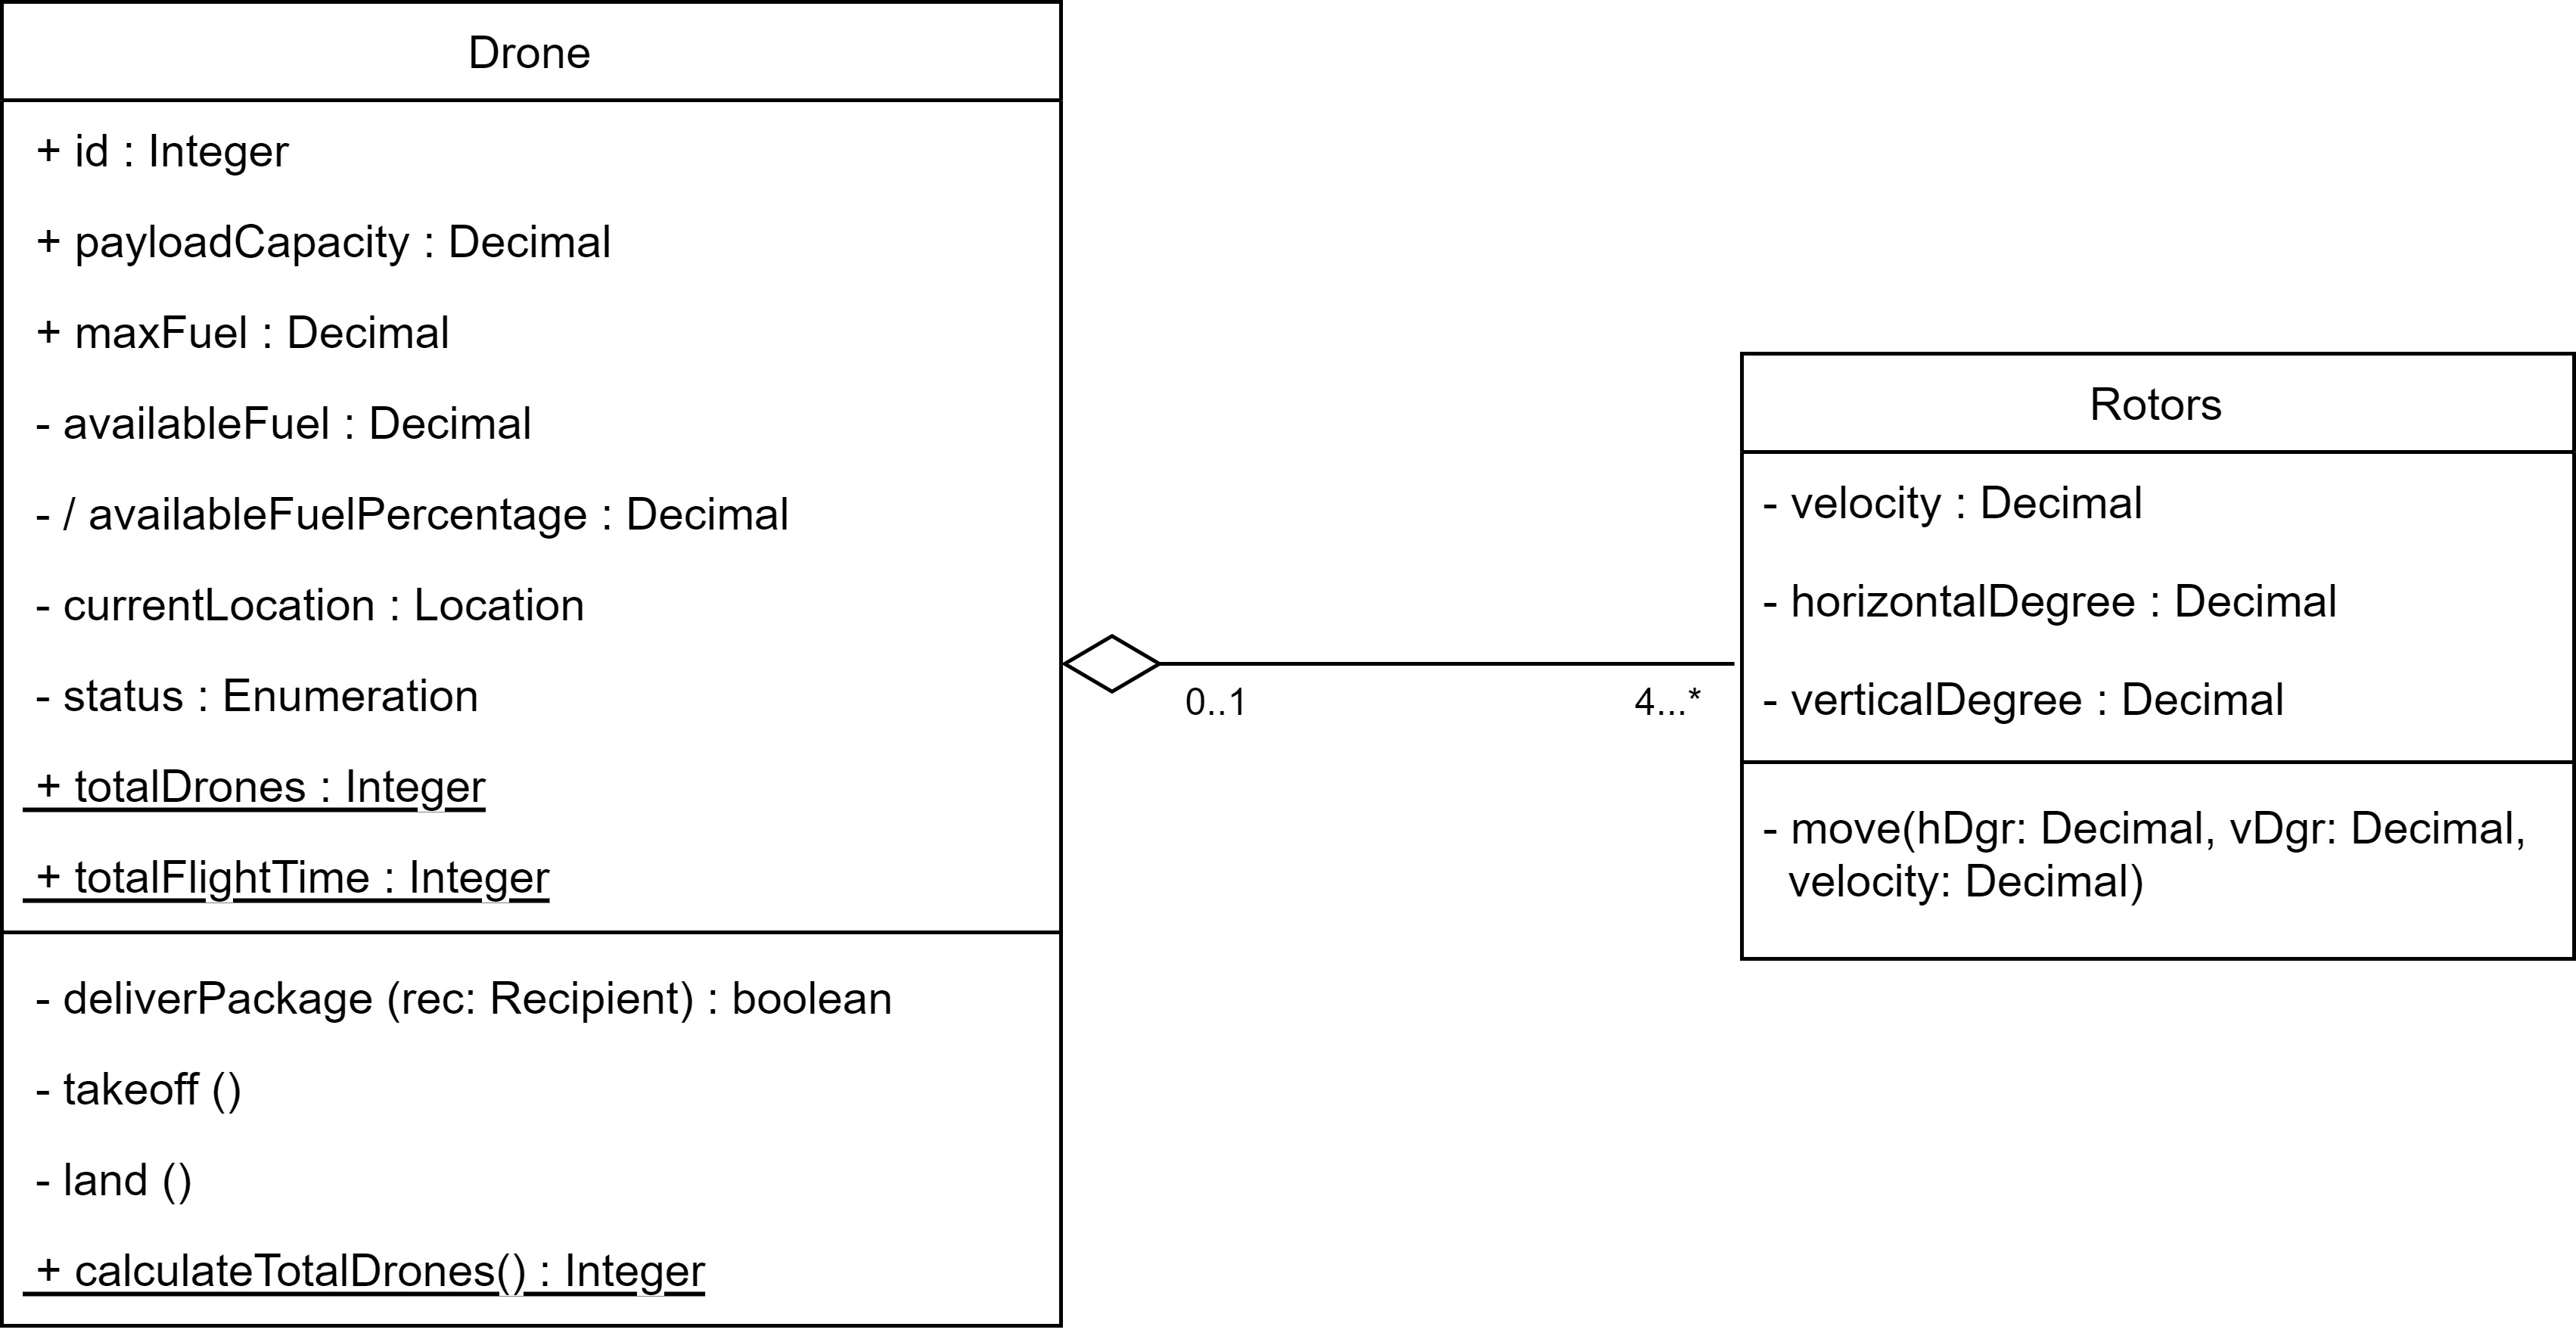
\includegraphics[width=0.8\textwidth]{figures/aggr_comp/aggr.jpg}
	\caption[Example aggregation]{Example of an aggregation}
	\label{fig:aggregation_example} 
\end{figure}


An example of an aggregation relationship involving a \texttt{Drone} class and a \texttt{Rotor} class is demonstrated in Figure \ref{fig:aggregation_example}. 
The \texttt{Drone} class contains a static attribute, \texttt{totalDrones}, which keeps track of the total number of drones, as well as a static operation, \texttt{calculateTotalDrones()}, which calculates this value. 
The class also includes a private operation, \texttt{sendDroneToRecipient()}, which is responsible for sending the drone to its intended recipient. 
The \texttt{Rotor} class, on the other hand, contains a private operation, \texttt{move()}, which is called by the \texttt{Drone} class's \texttt{sendDroneToRecipient()} operation and three private attributes, \texttt{velocity}, \texttt{horizontalDegree}, and \texttt{verticalDegree}, which control the movement of the drone in the air. \cite[p. 153]{uml}

The \texttt{Drone} class serves as the referencing class in this aggregation relationship and requires at least four \texttt{Rotor} instances to function properly. 
However, the drone has the capacity to utilize up to eight rotors at a time, as there are eight available slots for rotors on the drone. 
Each \texttt{Rotor} instance can be part of one or no drones at a given time.

If the \texttt{Rotor} instances become worn down or the weather conditions change, they can be replaced with new or specialized rotors. 
The destruction of a \texttt{Rotor} instance does not affect the existence of the \texttt{Drone}, and conversely, the destruction of a \texttt{Drone} instance does not affect the \texttt{Rotor} instances.

TODO: Qualifizierte Assoziation
   Darstellung einer ternären Assoziationn


\subsection{Composition}

In a UML class diagram, composition is a stronger form of relationship than aggregation and is represented by a solid line with a solid diamond at one end pointing towards the composite class. It represents a whole-part relationship between two classes, in which the whole class, known as the composite, is composed of one or more instances of the part class, known as the component.

The composite class is responsible for the lifecycle of the component class, meaning that the composite class creates and destroys the component class as needed. The component class cannot exist independently of the composite class and is tightly bound to the composite class. This is in contrast to an aggregation relationship, where the component class can exist independently of the aggregate class.

The multiplicities available for use in a composition relationship are restricted compared to those in an aggregation relationship. While a whole can have any number of parts, a part can only contribute to one whole. The multiplicity indicated by the solid diamond in a composition relationship is fixed at 0, 0..1, or 1. In many cases, the multiplicity is left out, which implies a multiplicity of 1. A multiplicity of 0 does not make sense in a composition relationship, and a multiplicity of 0..1 means that the parts are capable of existing independently for a certain period of time.(e.g. beispiel).
(e.g., the pineapple juice before it is mixed with the other ingredients of the cocktail).
 \cite[p. 153-154]{uml}

\begin{figure}[h]
\centering
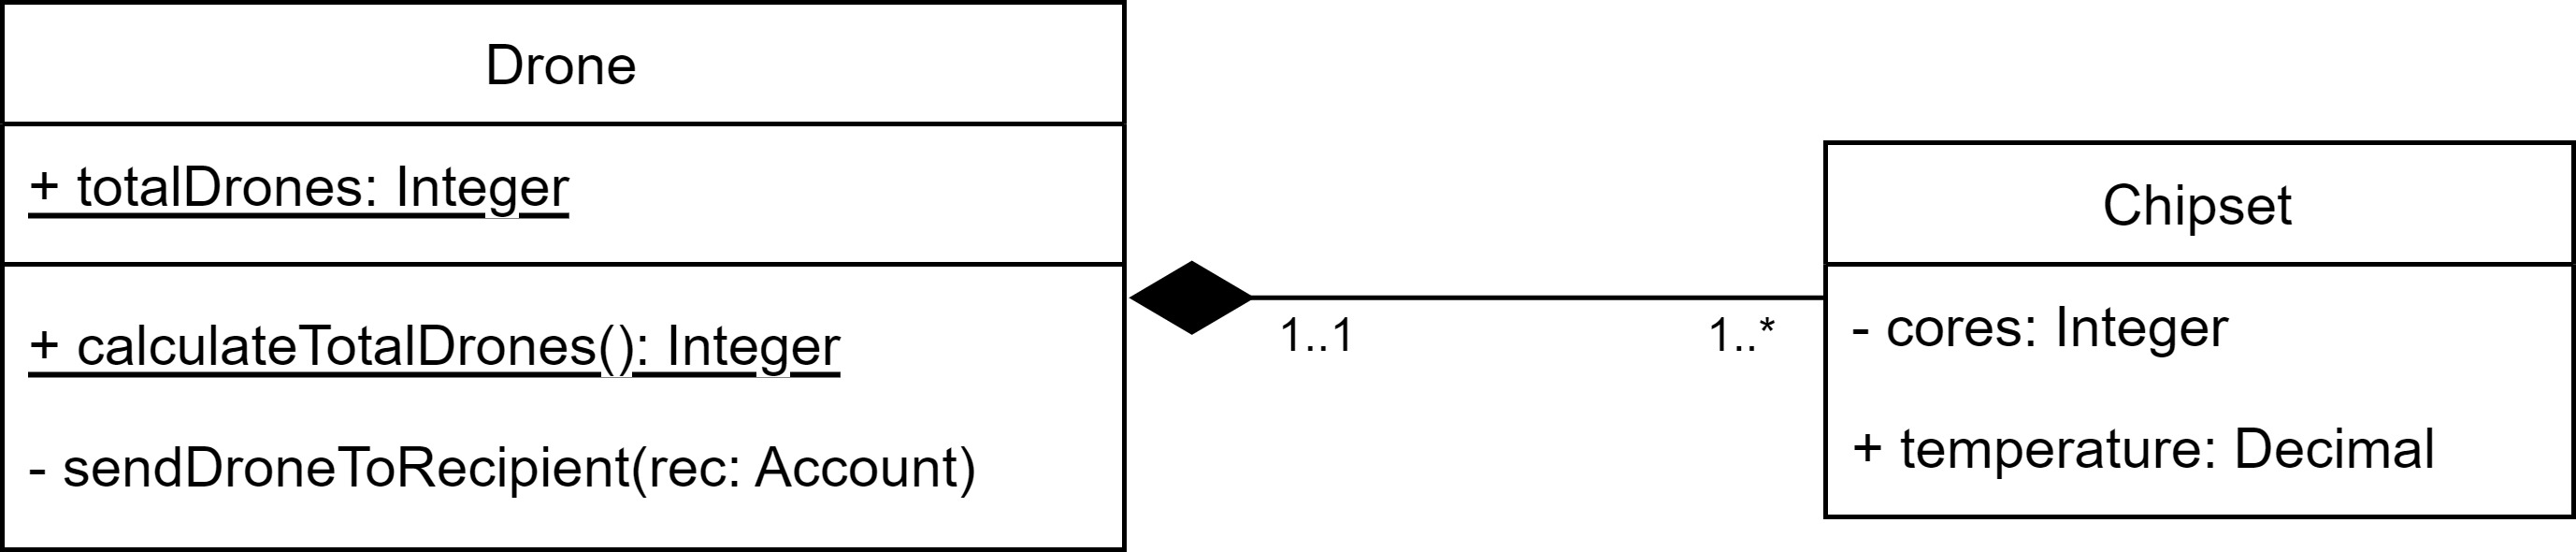
\includegraphics[width=0.8\textwidth]{figures/aggr_comp/comp.jpg}
\caption[Example composition]{Example of a composition}
\label{fig:composition_example}
\end{figure}


In Figure \ref{fig:composition_example}, an example of a composition relationship between the \texttt{Drone} class and the \texttt{Chipset} class is displayed. The \texttt{Chipset} class contains the private attribute \texttt{cores}, which stores information about the number of cores present in the chipset, and the public attribute \texttt{temperature}, which reflects the temperature of the chipset. As a vital component of the drone, the chipset is responsible for processing data and issuing commands to other parts of the drone. Without a functioning chipset, the drone would be unable to operate.

This design also incorporates an anti-theft concept, in which each chipset is uniquely bound to a specific drone. The number of chipsets used by the drone may vary based on their efficiency and the desired level of efficiency for the drone.


\section{Dependencies}

In UML, a dependency is a relationship between two elements in which one element (the client) uses or depends on another element (the supplier) for specification or implementation.
The dependency represents a semantic or structural relationship between the supplier and the client, indicating that the client is dependent on the supplier in some way (Booch, Rumbaugh, und Jacobson, 1998).
A dependency indicates that the connection between the two elements is at a higher level of abstraction than an association relationship.
Dependencies can be represented in various UML diagrams, including class diagrams, component diagrams, deployment diagrams, and use-case diagrams. 
To represent a dependency in a UML diagram, a dashed line with an open arrow pointing from the client to the supplier is used. 
In some cases, stereotypes may be used to show the precise nature of the dependency.

\vspace{1em}
{\RaggedRight
\begin{longtable} {|p{3.5cm}|p{3.25cm}|p{6.5cm}|}
		\hline
		\textbf{Type of dependency} & \textbf{Stereotype} & \textbf{Description} \\
		\hline
		Abstraction & «abstraction», «derive», «refine», or «trace» & Relates two model elements, or sets of model elements, that represent the same concept at different levels of abstraction, or from different viewpoints  \\ 
		\hline
		Binding & 	«bind» & Connects template arguments to template parameters to create model elements from templates \\ 
		\hline
		Realization & «realize» & 	Indicates that the client model element is an implementation of the supplier model element, and the supplier model element is the specification \\ 
		\hline
		Substitution & «substitute» & Indicates that the client model element takes the place of the supplier; the client model element must conform to the contract or interface that the supplier model element establishes  \\ 
		\hline
		Usage & «use», «call», «create», «instantiate», or «send» & Indicates that one model element requires another model element for its full implementation or operation  \\ 
		\hline
	\caption[Types of dependencies]{Types of dependency \cite{ibm_dependencies}}
	\label{tab:functional_req}
\end{longtable}
}

In cases where a client has a dependency on several suppliers, a connector (represented as a small black dot) can be used to model the dependency. This allows designers and developers to represent complex dependency relationships in a clear and concise manner, making it easier to understand the dependencies and interactions between different parts of a system.


\section{Foo Foo}
Hier folgt nun ein Listing, was basically Code ist. Und hier verlinke ich darauf: \autoref{lst:cleaning_impurity}.

\begin{lstlisting}[language=Python,caption={Pythonbeispiel nach Albrecht et al. \cite{albrecht_blueprints_2020}},captionpos=b,label={lst:cleaning_impurity}]
def sexyFunction(x):
	return x + 69
\end{lstlisting}	

\subsection{Foo Foo Foo}
\blindtext

\chapter{Bar}
\blindtext
\begin{figure}[h]
	\centering
	
\includegraphics[width=0.8\textwidth]{figures/pepe-example.png}
	\caption[Kürzerer Text für Abb.verzeichnis]{Ein äußerst wichtiger Frosch ist hier auf diesem Bild zu sehen. Diese Caption wäre zu lang für die Anzeige im Abb.verzeichnis, weswegen es diese eckigen Klammern gibt. Zitieren kannst du hier auch \cite{albrecht_blueprints_2020}}
	\label{fig:pepe_der_frosch} % UNTERHALB der \caption!
\end{figure}
\blindtext

\section{Bar Bar}
\blindtext
\\Es gibt eine wichtige Tabelle, nämlich die nun verlinkte \autoref{tab:frosch_tabelle_1}.

\subsection{Bar Bar Bar}
\blindtext
	\begin{table}[h]
	\centering
		\begin{tabular}{l|l|l}
		                        & Frosch         & Frosch        \\ \hline
		Strukturierter Frosch   & Datenabfrage   & Frosch Mining \\ \hline
		Unstrukturierter Frosch & Inhaltsabfrage & Text Frosch
		\end{tabular}%
	\caption[Eine Tabelle über Frösche]{Die Tabellencaption: Für Tabellen empfiehlt sich der https://www.tablesgenerator.com/}
	\label{tab:frosch_tabelle_1}
	\end{table}
\blindtext

\backmatter
%\listoftodos %remove if no longer needed

\printnoidxglossaries

% ACHTUNG: ursprüngl: alpha, aber das erzeugt keine Links
\bibliographystyle{wmaainf}
%\bibliographystyle{alpha}
\bibliography{refs}
\clearpage %\cleardoublepage

%-----------------------------------------------------------------------------------------------------------------

% remove if not needed
\appendix
%\pagenumbering{Alph}
\chapter{Supplemental Information}\label{app:supplemental-information}
Hier könnte Ihr Anhang stehen!


%-----------------------------------------------------------------------------------------------------------------


\end{document}